\clearpage
\appendix
\section{Appendix}
\subsection{LLM Disclaimer}
The authors hereby declare the role of large language model (LLM) tools in the preparation of this manuscript: LLMs were solely utilized to assist with text polishing (including refining sentence structure, optimizing lexical expression, and enhancing language fluency) and **writing optimization** of the paper’s narrative content.  

It is explicitly emphasized that all core components of this research, which determine the originality, scientific validity, and academic value of the work, were independently completed by the research team through manual efforts. These components include, but are not limited to:  
\begin{itemize}
    \item The formulation and development of the overall research framework, core ideas, and logical structure of the study; 
    \item The design, coding, debugging, and validation of all algorithms and program codes involved in the research;  
    \item The design of experimental protocols, collection and preprocessing of experimental data, execution of experiments, analysis and interpretation of experimental results, and verification of conclusions.  
\end{itemize}


The use of LLM tools did not involve any participation in the conception of research content, generation of technical solutions, implementation of experimental processes, or derivation of research conclusions. All content of this paper adheres to academic integrity standards, and the research team assumes full responsibility for the scientificity, authenticity, and originality of the work.



\newpage
\subsection{THEORETICAL PROOF OF ThEOREM \ref{theorem 1} and subsequent truncated SVD } \label{theorem1 derivation}
\paragraph{Problem Formulation.} 
Consider the optimization problem
\begin{equation}
   \min_{A,B} J(A,B) = \|ABX - Z\|_F^2,
\end{equation}
where the goal is to simplify the objective function $J(A,B)$ so that optimization with respect to $A$ and $B$ becomes more tractable. The key idea is to exploit the structure of the matrix $X$, particularly its row space.

\paragraph{Assumption.} 
To ensure that the following projection operations are well-defined, we assume that $X$ has full row rank, because in practice a small ridge parameter $\lambda$ will be introduced and $L_\ell=(H_\ell+\lambda I)^{-1/2}$.
This assumption is reasonable since the activation matrix $X$ typically has far more columns than rows. If $X$ is a $p \times n$ matrix with $p \ll n$, then $\mathrm{rank}(X) = p$, which guarantees that $XX^\top$ is invertible.

\paragraph{Orthogonal Projection Operator.} 
We define the projection matrix
\begin{equation}
   P = X^\top(XX^\top)^{-1}X,
\end{equation}
which is an $n \times n$ orthogonal projector mapping any row vector in $\mathbb{R}^n$ onto the row space of $X$. For any matrix $Y$ with $n$ columns, the product $YP$ projects each row of $Y$ onto the row space of $X$. 

The matrix $P$ satisfies several important properties:
\begin{itemize}
    \item \textbf{Symmetry:} $P^\top = P$, since $XX^\top$ is symmetric and so is its inverse.
    \item \textbf{Idempotence:} $P^2 = P$, which follows by direct calculation.
    \item \textbf{Projection property:} For any matrix of the form $CX$, right multiplication by $P$ leaves it unchanged, i.e., $(CX)P = CX$. In particular, $ABX$ belongs to this class.
\end{itemize}

\paragraph{Decomposition of $Z$.} 
We decompose $Z$ into components lying in the row space of $X$ and its orthogonal complement:
\begin{equation}
   Z_P = ZP, \qquad Z_\perp = Z(I-P).
\end{equation}
Clearly,
\begin{equation}
   Z = ZP + Z(I-P) = Z_P + Z_\perp,
\end{equation}
where $Z_P$ is the projection of $Z$ onto the row space of $X$, and $Z_\perp$ is the projection onto its orthogonal complement. Moreover, $Z_\perp P = 0$.

\paragraph{Reformulated Objective.}
Using this decomposition, we expand the objective:
    \begin{equation}
\begin{aligned}
   J(A,B) &= \|ABX - Z\|_F^2 \\
          &= \|ABX - (Z_P + Z_\perp)\|_F^2 \\
          &= \|(ABX - Z_P) - Z_\perp\|_F^2.
\end{aligned}
\end{equation}
Let $U = ABX - Z_P$ and $V = Z_\perp$. Since $U$ lies in the row space of $X$ and $V$ lies in its orthogonal complement, they are orthogonal, i.e., $\mathrm{Tr}(U^\top V) = 0$. By the Pythagorean theorem for the Frobenius norm, we obtain
\begin{equation}
   J(A,B) = \|ABX - Z_P\|_F^2 + \|Z_\perp\|_F^2.
   \label{eq jab}
\end{equation}

%  其中$\|Z\perp\|_F^2$ 是个常数此时我们将$P=X^\top (XX^\top)^{-1}X$代入公式\ref{eq jab} 从而得到 
By the premise, we start from
\begin{equation}
J(A,B) \;=\; \|\,ABX - ZX^\top(XX^\top)^{-1}X\,\|_F^2 \;=\; \|\,U X - ZP\,\|_F^2,
\qquad where\, U=AB .
\label{eq:start}
\end{equation}

\paragraph{Step 1: Projection reduction is tight up to a constant.}
Decompose $Z$ into its components on the row space of $X$ and its orthogonal complement:
\begin{equation}
Z \;=\; ZP \;+\; Z(I-P) \;=:\; Z_P + Z_\perp,
\qquad Z_\perp P = 0 .
\end{equation}
Since $UX$ lies in the row space of $X$, we have $(UX)P=UX$. Therefore,
\begin{align}
\|UX - Z\|_F^2
&= \|UX - (Z_P + Z_\perp)\|_F^2
= \|(UX - Z_P) - Z_\perp\|_F^2 \nonumber\\
&= \|UX - Z_P\|_F^2 + \|Z_\perp\|_F^2 
\quad\text{(orthogonality in the row/orthogonal subspaces).}
\label{eq:pyth}
\end{align}
Thus minimizing $\|UX - ZP\|_F^2$ is equivalent to minimizing $\|UX - Z\|_F^2$, since they differ by the constant $\|Z_\perp\|_F^2$ independent of $U$. Hence \eqref{eq:start} is a valid surrogate objective.

\paragraph{Step 2: Whitening reformulation.}
Let $M=ZX^\top\in\mathbb{R}^{m\times p}$. Expand the Frobenius norm using trace identities:
\begin{align}
\|UX - ZP\|_F^2
&= \|UX - ZP\|_F^2
= \|(UX - Z)P\|_F^2
= \operatorname{tr}\!\big((UX - Z)P(UX - Z)^\top\big) \nonumber\\
&= \operatorname{tr}(UXX^\top U^\top) - 2\,\operatorname{tr}(UXPZ^\top) + \operatorname{tr}(ZPZ^\top) \nonumber\\
&= \operatorname{tr}(UHU^\top) - 2\,\operatorname{tr}(UM^\top) + \operatorname{tr}(ZPZ^\top).
\label{eq:expand}
\end{align}
Because $H\succ0$, its symmetric square roots $H^{\pm 1/2}$ exist and are invertible. Using
\begin{equation}
\operatorname{tr}(UHU^\top)=\|UH^{1/2}\|_F^2,
\qquad
\operatorname{tr}(UM^\top)=\langle UH^{1/2},\, MH^{-1/2}\rangle_F,
\end{equation}
we can complete the square:
\begin{align}
\|UX - ZP\|_F^2
&= \|UH^{1/2}\|_F^2 - 2\langle UH^{1/2}, MH^{-1/2}\rangle_F + \operatorname{tr}(ZPZ^\top) \nonumber\\
&= \|UH^{1/2} - MH^{-1/2}\|_F^2 
\;+\; \Big(\operatorname{tr}(ZPZ^\top) - \|MH^{-1/2}\|_F^2\Big).
\label{eq:completed-square}
\end{align}
The parenthetical term is independent of $U$. Therefore the minimizers of \eqref{eq:start} are exactly the minimizers of
\begin{equation}
\min_{\operatorname{rank}(U)\le r}\ \big\|UH^{1/2} - MH^{-1/2}\big\|_F^2 .
\end{equation}
At this point, we have completed the proof of Theorem \ref{theorem 1}. Subsequently, we will perform low-rank approximation based on this.

\paragraph{Step 3: Invertible change of variables and rank preservation.}
Define the change of variables
\begin{equation}
V \;=\; U H^{1/2}, 
\qquad
L \;=\; H^{-1/2}.
\end{equation}
Since $H^{1/2}$ is invertible, $\operatorname{rank}(V)=\operatorname{rank}(U)$, so the rank constraint is preserved. The problem is thus equivalent to
\begin{equation}
\min_{\operatorname{rank}(V)\le r}\ \|\,V - ML\,\|_F^2 .
\end{equation}
This proves the desired whitening equivalence: minimizing $\|UX - ZP\|_F^2$ over rank-$r$ $U$ is equivalent to minimizing $\|V - ML\|_F^2$ over rank-$r$ $V$, with the bijection between minimizers given by $U^\star = V^\star H^{-1/2}$.


\newpage
\subsection{THEORETICAL PROOF OF THEOREM \ref{theorem2}: Fixed-Subspace First-Order Approximation for Truncation Ratios}
\label{app:fsfoa}
\label{theorem2 derivation}

\paragraph{Setup.}
Let $S\in\mathbb{R}^{m\times n}$ with singular value decomposition $S=U\Sigma V^\top$, and fix a target rank $r\in\{1,\dots,\min(m,n)-1\}$. Denote
\[
U_r:=U_{[:,1:r]},\quad V_r:=V_{[:,1:r]},\qquad
P_L:=I-U_rU_r^\top,\quad P_R:=I-V_rV_r^\top.
\]
Given a direction $D\in\mathbb{R}^{m\times n}$ and a scalar $\beta\in[0,1]$, define the affine path
\begin{equation}\label{eq:affine_path}
G(\beta):=S+\beta D.
\end{equation}
Let $\|\cdot\|_F$ be the Frobenius norm, $\|\cdot\|_2$ the spectral norm, and let $\sigma_1(\cdot)\ge\cdots$ denote singular values.

\paragraph{True tail energy and ratio.}
By the Eckart--Young--Mirsky theorem,
\begin{equation}\label{eq:tail_energy}
E(\beta)\ :=\ \min_{\operatorname{rank}(Q)\le r}\ \|G(\beta)-Q\|_F^2\ =\ \sum_{i>r}\sigma_i\!\big(G(\beta)\big)^2.
\end{equation}
We call $\sqrt{E(\beta)}$ the \emph{tail (Frobenius) norm} of $G(\beta)$ at rank $r$. The corresponding \emph{tail ratio} is
\begin{equation}\label{eq:tail_ratio}
\rho(\beta)\ :=\ \frac{\sqrt{E(\beta)}}{\ \|G(\beta)\|_F\ }.
\end{equation}

\paragraph{Fixed-subspace first-order approximation (FS-FOA).}
Freeze the leading rank-$r$ subspaces at $\beta=0$ (those of $S$), and approximate the tail by the projection onto the fixed orthogonal complement:
\begin{equation}\label{eq:fsfoa_tail_energy}
\widetilde E(\beta)\ :=\ \big\|\,P_L\,G(\beta)\,P_R\,\big\|_F^2
\ =\ \big\|\,S_\perp+\beta D_\perp\,\big\|_F^2, \quad
S_\perp:=P_LSP_R,\ \ D_\perp:=P_LDP_R.
\end{equation}
The \emph{FS-FOA tail ratio} is then
\begin{equation}\label{eq:fsfoa_ratio}
\widetilde\rho(\beta)\ :=\ \frac{\|S_\perp+\beta D_\perp\|_F}{\|S+\beta D\|_F}.
\end{equation}

\paragraph{Assumption (spectral gap and small perturbation).}
Let the spectral gap at $r$ be
\begin{equation}\label{eq:gap_assump}
\delta\ :=\ \sigma_r(S)-\sigma_{r+1}(S)\ >\ 0,
\end{equation}
and assume the relative perturbation is small:
\begin{equation}\label{eq:tau_assump}
\tau\ :=\ \frac{\beta\,\|D\|_2}{\delta}\ \le\tau_0, \qquad \text{for some sufficiently small }\tau_0\in(0,1).
\end{equation}

\paragraph{Theorem (FS-FOA is first-order accurate for the tail energy).}
Under \eqref{eq:gap_assump}--\eqref{eq:tau_assump}, there exist absolute constants $C_1,C_2>0$ such that for all $\beta\in[0,1]$,
\begin{equation}\label{eq:fsfoa_main_bound}
E(\beta)\ =\ \|S_\perp+\beta D_\perp\|_F^2\ +\ R_E(\beta),
\qquad
\big|R_E(\beta)\big|\ \le\ C_1\,\tau^2\Big(\|S\|_F^2+\beta^2\|D\|_F^2\Big).
\end{equation}
In particular, the discrepancy between the true tail energy and its FS-FOA surrogate is \emph{second order} in $\tau$.

\paragraph{Corollary (FS-FOA is first-order accurate for the tail ratio).}
With the same assumptions, there exists $C'>0$ such that
\begin{equation}\label{eq:ratio_bound}
\big|\rho(\beta)-\widetilde\rho(\beta)\big|\ \le\ C'\,\tau^2
\ =\ O\!\left(\frac{\beta^2\|D\|_2^2}{\delta^2}\right).
\end{equation}
Hence $\widetilde\rho(\beta)$ is a first-order accurate approximation to the true ratio $\rho(\beta)$.

\paragraph{Proof sketch of \eqref{eq:fsfoa_main_bound}.}
Let $U_r(\beta),V_r(\beta)$ be the leading $r$-dimensional singular subspaces of $G(\beta)$ and $P_L(\beta)=I-U_r(\beta)U_r(\beta)^\top$, $P_R(\beta)=I-V_r(\beta)V_r(\beta)^\top$ their orthogonal complements. Standard Davis--Kahan/Wedin perturbation bounds imply
\begin{equation}\label{eq:proj_bounds}
\|P_L(\beta)-P_L\|_2\ \lesssim\ \tau,\qquad \|P_R(\beta)-P_R\|_2\ \lesssim\ \tau.
\end{equation}
Because $E(\beta)=\|P_L(\beta)G(\beta)P_R(\beta)\|_F^2$, write $P_L(\beta)=P_L+E_L$, $P_R(\beta)=P_R+E_R$ with $\|E_{L/R}\|_2=O(\tau)$ and expand:
\[
P_L(\beta)G(\beta)P_R(\beta)
=(P_L+E_L)(S+\beta D)(P_R+E_R)
= P_L(S+\beta D)P_R\ +\ \mathcal{E},
\]
where the Frobenius norm of the remainder satisfies $\|\mathcal{E}\|_F=O\!\big(\tau\,\|G(\beta)\|_F\big)$ by the block structure induced by $(U_r,V_r)$. Squaring norms yields
\[
E(\beta)=\|P_LGP_R\|_F^2 + O\!\big(\tau^2\|G(\beta)\|_F^2\big)
=\|S_\perp+\beta D_\perp\|_F^2 + O\!\big(\tau^2(\|S\|_F^2+\beta^2\|D\|_F^2)\big),
\]
which is \eqref{eq:fsfoa_main_bound}. The corollary \eqref{eq:ratio_bound} follows by dividing by $\|G(\beta)\|_F^2$ and using $\sqrt{1+x}=1+O(x)$ for small $x$.

\paragraph{Closed form for the FS-FOA ratio and its stationary condition.}
Both numerator and denominator of \eqref{eq:fsfoa_ratio} are quadratic polynomials in $\beta$:
\begin{equation}\label{eq:num_quad}
\|S_\perp+\beta D_\perp\|_F^2\ =\ a+2b\,\beta+c\,\beta^2,
\end{equation}
\begin{equation}\label{eq:den_quad}
\|S+\beta D\|_F^2\ =\ A+2B\,\beta+C\,\beta^2,
\end{equation}
where
\begin{equation}\label{eq:abc_defs}
a:=\|S_\perp\|_F^2,\quad b:=\langle S_\perp,D_\perp\rangle,\quad c:=\|D_\perp\|_F^2,\qquad
A:=\|S\|_F^2,\quad B:=\langle S,D\rangle,\quad C:=\|D\|_F^2.
\end{equation}
Let
\begin{equation}\label{eq:phi_def}
\phi(\beta):=\widetilde\rho(\beta)=\sqrt{\frac{a+2b\beta+c\beta^2}{A+2B\beta+C\beta^2}}.
\end{equation}
Since the square root is monotone, $\arg\min\phi$ coincides with $\arg\min$ of the squared ratio. Differentiating and simplifying gives the \emph{quadratic} stationary equation
\begin{equation}\label{eq:stationary_quadratic}
(cB-bC)\,\beta^2\ +\ (cA-aC)\,\beta\ +\ (bA-aB)\ =\ 0.
\end{equation}
\emph{Selection rule.} Solve \eqref{eq:stationary_quadratic}, keep real roots in $[0,1]$, add the boundaries $\{0,1\}$, evaluate $\widetilde\rho(\beta)$ on this candidate set, and choose the minimizer $\beta^*\in[0,1]$. In applications with a trade-off parameter $\alpha\ge 0$, one uses the bijection
\begin{equation}\label{eq:alpha_beta}
\beta=\frac{\alpha}{1+\alpha}\quad\Longleftrightarrow\quad \alpha=\frac{1}{1-\beta}-1,
\end{equation}
so that $\alpha^*=\frac{1}{\beta^*}-1$.

\paragraph{When is FS-FOA accurate.}
Accuracy is controlled by $\tau=\beta\|D\|_2/\delta$. When $\tau\ll 1$ (e.g., $\tau\lesssim 0.5$), the error in \eqref{eq:fsfoa_main_bound}--\eqref{eq:ratio_bound} is second order and the stationary points of $\widetilde\rho$ reliably approximate those of $\rho$. In near-degenerate cases (small spectral gap or large $D$), one may constrain $\beta\le\beta_{\max}<1$ or apply a mild shrinkage to the selected $\beta^*$; a one-step refinement that recomputes the leading subspaces at $G(\beta^*)$ further reduces the residual error.

\paragraph{Interpretation.}
The numerator in \eqref{eq:fsfoa_ratio} measures the energy that would be \emph{discarded} by rank-$r$ truncation (tail) when measured in the fixed orthogonal complement of the leading subspaces of $S$; the denominator measures the \emph{total} energy. The quadratic form \eqref{eq:stationary_quadratic} encodes the balance between tail alignment $(a,b,c)$ and total alignment $(A,B,C)$, yielding a closed-form, one-dimensional selection of $\beta$ (hence $\alpha$) that minimizes the truncation ratio to first order.



\newpage
\subsection{Quantitative Results}
% 需要的宏包：
% \usepackage{booktabs}
% \usepackage{multirow}
% \usepackage[table]{xcolor} % 行底色

\begin{table}[h]
  \centering
  \small
  \caption{Performance of Compressed Llama-2-7B Across Benchmarks and Compression Ratios.}
  \begin{tabular}{llrrrrrrrr}
    \toprule
    Ratio & Method & WikiText-2 & PTB & C4 & ARC\_e & WinoG. & HellaS. & PIQA & Average \\
    \midrule
    0   & Original & 5.68  & 8.35   & 7.34   & 74.62 & 69.22 & 76.00 & 79.11 & 68.85 \\
    \midrule
    \multirow{6}{*}{0.4}
      & SVD       & 39661.03 & 69493.00 & 56954.00 & 26.39 & 48.62 & 25.64 & 52.99 & 38.41 \\
      & FWSVD     & 8060.35  & 9684.10  & 7955.21  & 26.05 & 50.20 & 25.70 & 52.39 & 38.59 \\
      & ASVD      & 1609.32  & 7319.49  & 1271.85  & 26.81 & 49.49 & 25.83 & 53.81 & 38.99 \\
      & SVD-LLM   & 161.11   & 719.44   & 61.95    & 36.99 & 56.04 & 30.49 & 56.96 & 45.12 \\
      & AdaSVD    & 14.76    & 304.62   & 56.98    & 41.12 & 58.17 & 31.75 & 58.49 & 47.38 \\
      \rowcolor{gray!12}
      & Ours      & 11.35    & 217.20   & 40.57    & 43.27 & 57.77 & 32.14 & 58.92 & \textbf{48.03} \\
    \midrule
    \multirow{6}{*}{0.5}
      & SVD       & 53999.48 & 39207.00 & 58558.00 & 25.80 & 47.36 & 25.55 & 52.67 & 37.85 \\
      & FWSVD     & 8173.21  & 8615.71  & 8024.67  & 25.84 & 48.70 & 25.64 & 52.83 & 38.25 \\
      & ASVD      & 6977.57  & 15539.44 & 4785.15  & 25.13 & 49.17 & 25.48 & 52.94 & 38.18 \\
      & SVD-LLM   & 272.19   & 1772.91  & 129.66   & 31.65 & 51.14 & 28.38 & 54.57 & 41.44 \\
      & AdaSVD    & 25.58    & 593.14   & 113.84   & 34.18 & 54.06 & 28.88 & 55.50 & 43.16 \\
      \rowcolor{gray!12}
      & Ours      & 14.02    & 95.48    & 48.94    & 35.56 & 55.80 & 29.58 & 56.58 & \textbf{44.38} \\
    \midrule
    \multirow{6}{*}{0.6}
      & SVD       & 65186.67 & 79164.00 & 70381.00 & 24.49 & 51.85 & 25.40 & 53.16 & 38.73 \\
      & FWSVD     & 27213.30 & 24962.80 & 47284.87 & 25.38 & 48.46 & 25.61 & 51.96 & 37.85 \\
      & ASVD      & 10003.57 & 15530.19 & 9983.83  & 26.68 & 48.86 & 25.76 & 51.80 & 38.28 \\
      & SVD-LLM   & 89.90    & 2052.89  & 561.00   & 26.73 & 47.43 & 26.89 & 53.48 & 38.63 \\
      & AdaSVD    & 50.33    & 1216.95  & 239.18   & 28.20 & 51.22 & 27.36 & 52.83 & 39.90 \\
      \rowcolor{gray!12}
      & Ours      & 23.89    & 334.67   & 100.42   & 31.02 & 52.01 & 30.38 & 54.62 & \textbf{42.01} \\
    \bottomrule
  \end{tabular}
  \label{tab:27b}
\end{table}

% preamble:
% \usepackage{booktabs}
% \usepackage[table]{xcolor}

\begin{table}[h]
\centering
\setlength{\tabcolsep}{5pt}
\caption{PPL and accuracy of LLaMA-3-8B across compression ratios comparing SVD-LLM and Ours.}
\resizebox{\linewidth}{!}{
\begin{tabular}{c l r r r r r r r r r}
\toprule
Ratio & Method & \multicolumn{1}{c}{WikiText-2 (PPL)\,$\downarrow$} & \multicolumn{1}{c}{Openb\,$\uparrow$} & \multicolumn{1}{c}{ARC\_c\,$\uparrow$} & \multicolumn{1}{c}{ARC\_e\,$\uparrow$} & \multicolumn{1}{c}{WinoG.\,$\uparrow$} & \multicolumn{1}{c}{HellaS.\,$\uparrow$} & \multicolumn{1}{c}{PIQA\,$\uparrow$} & \multicolumn{1}{c}{MathQA\,$\uparrow$} & \multicolumn{1}{c}{Mean\,$\uparrow$} \\
\midrule
\multirow{2}{*}{0.2}
& SVD-LLM & 13.87 & 0.242 & 0.278 & 0.579 & 0.648 & 0.393 & 0.664 & 0.259 & 0.438 \\
% \rowcolor{gray!10}
& Ours    & \textbf{11.49} & \textbf{0.252} & \textbf{0.284} & \textbf{0.593} & \textbf{0.658} & \textbf{0.393} & \textbf{0.671} & \textbf{0.268} & \textbf{0.446} \\
\midrule
\multirow{2}{*}{0.4}
& SVD-LLM & 80.46 & 0.134 & 0.193 & 0.325 & 0.523 & 0.274 & 0.548 & 0.208 & 0.315 \\
% \rowcolor{gray!10}
& Ours    & \textbf{23.30} & \textbf{0.162} & \textbf{0.196} & \textbf{0.340} & \textbf{0.554} & \textbf{0.296} & \textbf{0.552} & \textbf{0.218} & \textbf{0.331} \\
\midrule
\multirow{2}{*}{0.6}
& SVD-LLM & 729.46 & 0.104 & 0.207 & 0.272 & 0.521 & 0.264 & 0.529 & 0.211 & 0.301 \\
% \rowcolor{gray!10}
& Ours    & \textbf{63.09} & \textbf{0.136} & \textbf{0.219} & \textbf{0.285} & \textbf{0.534} & \textbf{0.278} & \textbf{0.535} & \textbf{0.225} & \textbf{0.316} \\
\midrule
\multirow{2}{*}{0.8}
& SVD-LLM & 6971.65 & 0.120 & \textbf{0.207} & 0.259 & 0.503 & 0.258 & 0.531 & 0.201 & 0.297 \\
% \rowcolor{gray!10}
& Ours    & \textbf{181.84} & \textbf{0.140} & 0.203 & \textbf{0.281} & \textbf{0.520} & \textbf{0.259} & \textbf{0.539} & \textbf{0.208} & \textbf{0.307} \\
\bottomrule
\end{tabular}
}

\label{tab:38b}
\end{table}

We have supplemented detailed experimental results on different compression ratios for LLama-2 and LLama-3. As shown in Table~\ref{tab:27b} and Table~\ref{tab:38b}, our method consistently achieves superior results across different compression ratios. Especially under extreme compression ratio conditions, such as Llama3-8B at a compression ratio of 0.8, our method outperforms the SVD-LLM method by nearly two orders of magnitude on the Perplexity metric.


\newpage
\subsection{Visualization of Self-Adaptation Beta}
To clarify the impact of different beta coefficients on the low-rank property of the optimization objective in Section~\ref{sec:cealc}, we visualized the compression of the k-proj Linear layer of the 14th layer of LLama3-8B. As shown in Figure~\ref{fig:different beta ratio}, beta affects the low-rank property of the optimization objective. The difference between the most suitable beta and the worst beta within the range of [0,1] is significant. When beta = 0.95, as shown in the first subfigure, the proportion  of discarded spectral energy is 7\%, while when beta = 0.4, only 4.7\% of the spectral energy is lost.
\begin{figure}[ht]
    \centering
    % 裁剪图片边缘可能存在的白色区域（根据实际情况调整参数）
        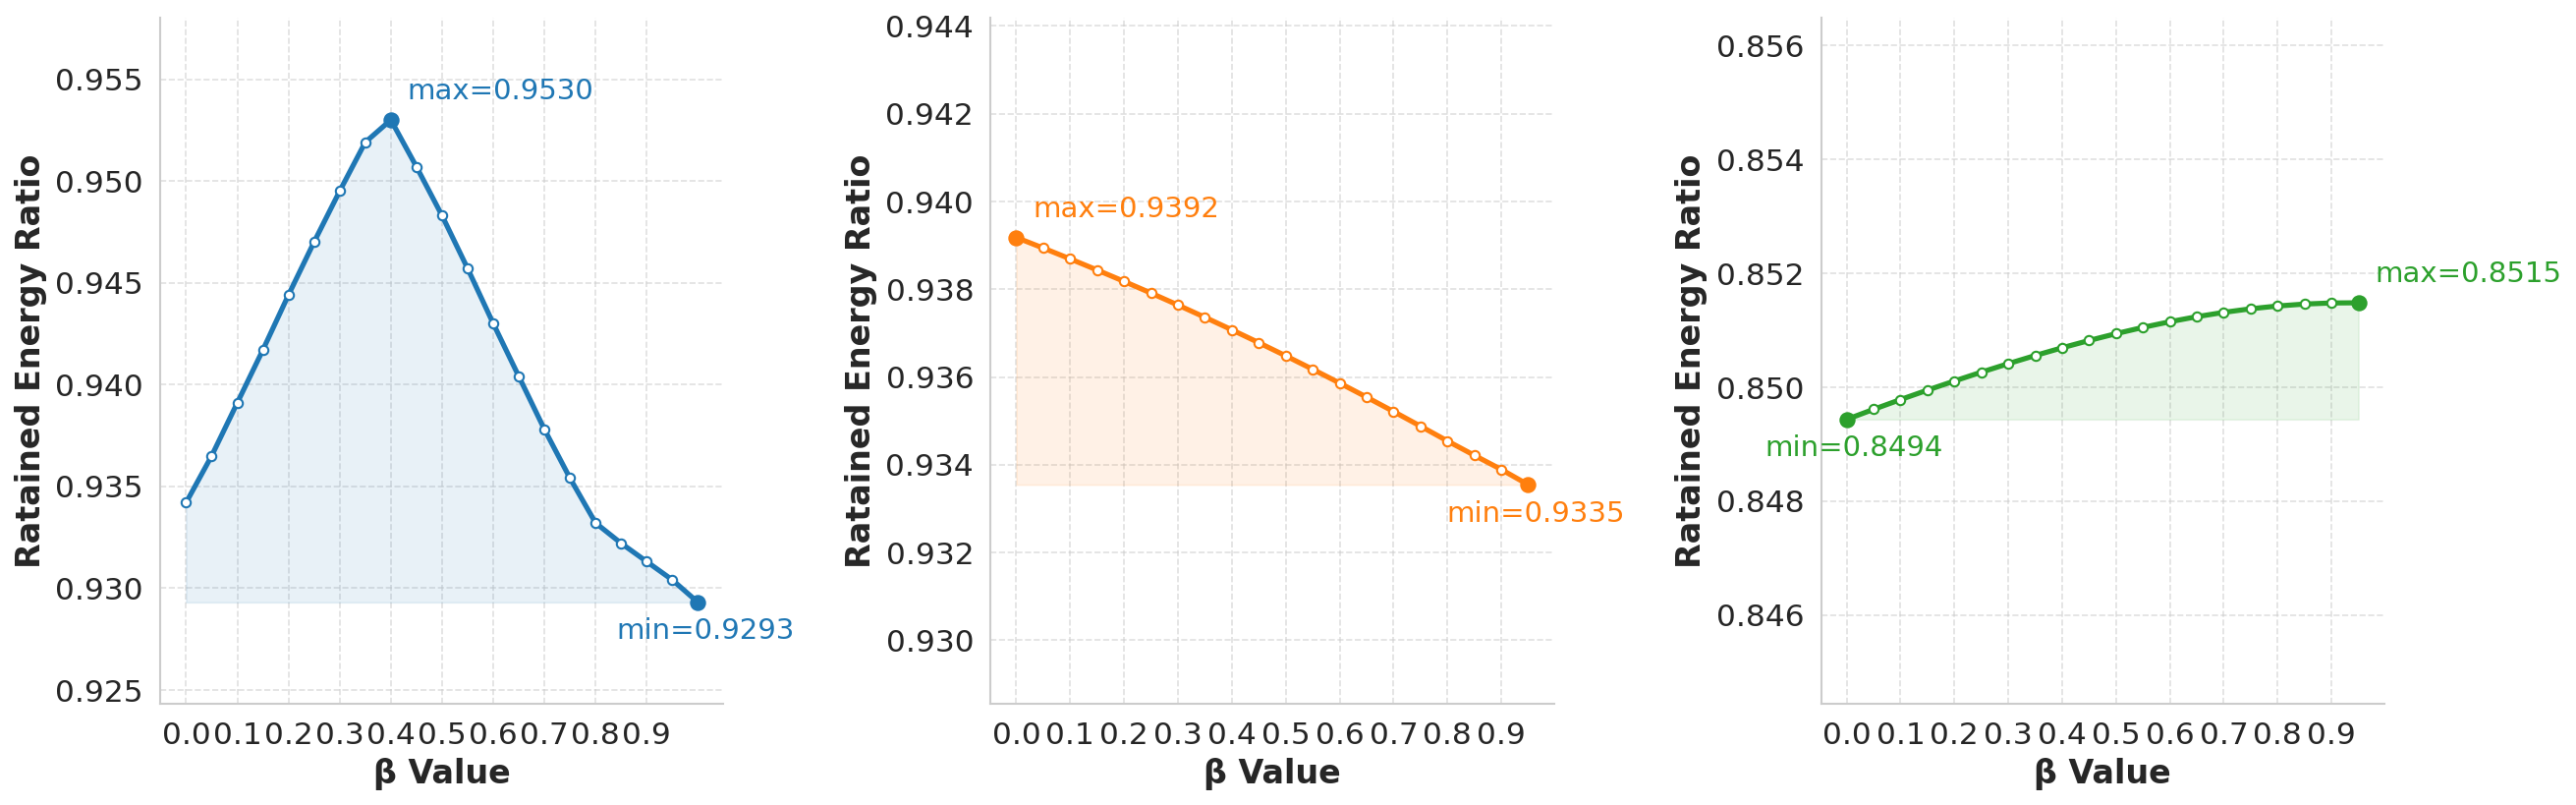
\includegraphics[width=1\linewidth]{figs/three_ratio_of_differnet_beta.png}
    % 调整标题与图片的距离
    \caption{ Using different beta coefficients for the k-proj of LLama3-8B at layer 14, layer 3 and layer 20 after the SVD in Equation~\ref{eq:final svd}, the proportion of retained energy at rank-1228.}
    \label{fig:different beta ratio}  % 标签使用冒号分隔符，符合LaTeX规范
    % 调整图与下文的距离
    \end{figure}

We visualized in Figure~\ref{fig:optiminal beta} the Self-Adaptation beta coefficients of the odd k-proj layers of the LLama3-8B model under the condition of a compression ratio of 0.4. As can be observed from the figure, in the shallow layers of the network, beta tends to be small. As the number of layers deepens, the optimal beta continuously increases. In the last few layers, a downward trend appears.
\begin{figure}[ht]
    \centering
    % 裁剪图片边缘可能存在的白色区域（根据实际情况调整参数）
        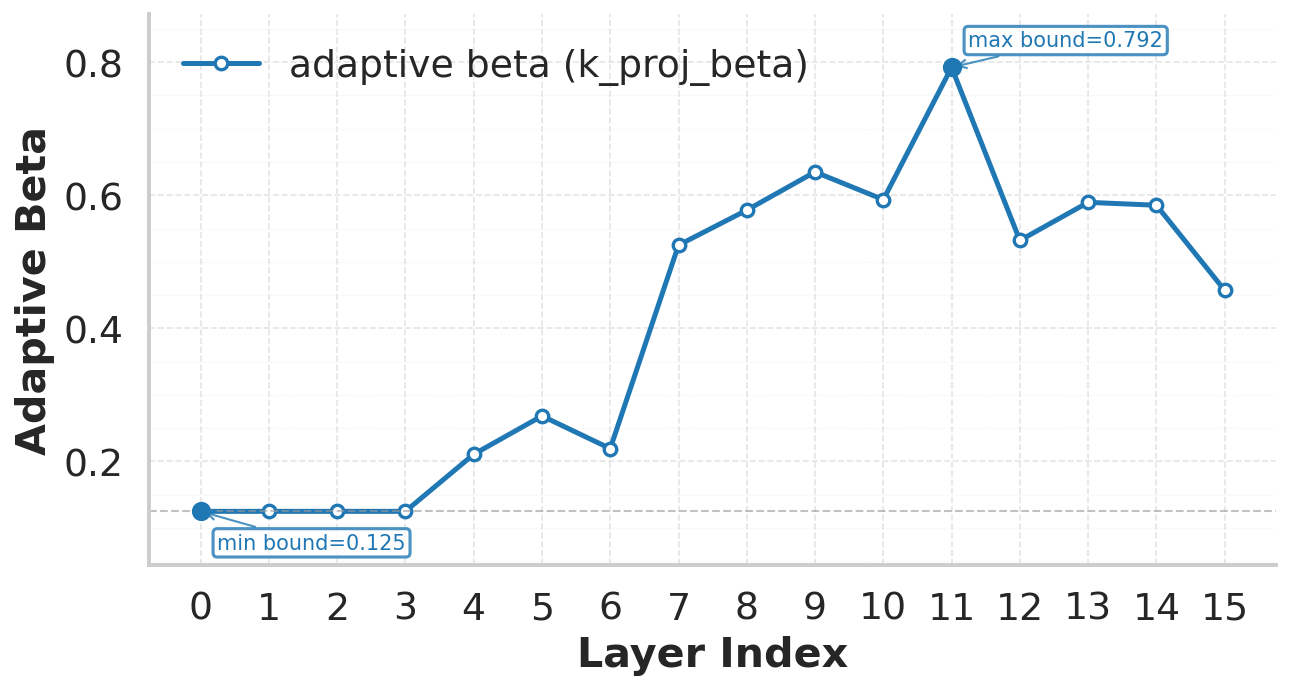
\includegraphics[width=1\linewidth]{figs/adaptive_beta_by_layer.png}
    % 调整标题与图片的距离
    \caption{The visualization of the optimal beta values obtained from k-proj of odd-numbered layers on LLaMA2-7B.}
    \label{fig:optiminal beta}  % 标签使用冒号分隔符，符合LaTeX规范
    % 调整图与下文的距离
    \end{figure}

\newpage
\subsection{Performance on more architectures and more challenging tasks}

\begin{table*}[h]
\centering
\caption{{Performance comparison of different compression methods on LLaMA3.1 and Qwen2.5 architectures at 0.2 compression rate across multiple benchmarks. Results are reported for 7 zero-shot tasks (ZeroShot\textsuperscript{7}), long-context understanding (LongEval), code generation (HumanEval), and mathematical reasoning (GSM8K).}}
\label{tab:qwen}
\begin{tabular}{l|l|cccc}
\hline
\textbf{Model} & \textbf{Method} & \textbf{ZeroShot\textsuperscript{7}} & \textbf{LongEval} & \textbf{HumanEval} & \textbf{GSM8K} \\
\hline
\multirow{4}{*}{LLaMA3.1-8B}
 & FP & 0.61 & 0.41 & 0.35 & 0.15 \\
 & ASVD & 0.49 & 0.33 & 0.15 & 0.06 \\
 & SVD-LLM & 0.57 & 0.37 & 0.27 & 0.10 \\
 & \textbf{Ours} & \textbf{0.59} & \textbf{0.39} & \textbf{0.33} & \textbf{0.13} \\
\hline
\multirow{4}{*}{LLaMA3.1-70B}
 & FP & 0.67 & 0.49 & 0.55 & 0.37 \\
 & ASVD & 0.54 & 0.39 & 0.32 & 0.26 \\
 & SVD-LLM & 0.63 & 0.45 & 0.47 & 0.32 \\
 & \textbf{Ours} & \textbf{0.66} & \textbf{0.48} & \textbf{0.52} & \textbf{0.35} \\
\hline
\multirow{4}{*}{Qwen2.5-7B}
 & FP & 0.60 & 0.58 & 0.66 & 0.71 \\
 & ASVD & 0.50 & 0.49 & 0.41 & 0.42 \\
 & SVD-LLM & 0.56 & 0.55 & 0.55 & 0.64 \\
 & \textbf{Ours} & \textbf{0.58} & \textbf{0.57} & \textbf{0.63} & \textbf{0.69} \\
\hline
\multirow{4}{*}{Qwen2.5-32B}
 & FP & 0.65 & 0.79 & 0.55 & 0.72 \\
 & ASVD & 0.52 & 0.61 & 0.37 & 0.44 \\
 & SVD-LLM & 0.61 & 0.73 & 0.46 & 0.63 \\
 & \textbf{Ours} & \textbf{0.64} & \textbf{0.76} & \textbf{0.51} & \textbf{0.68} \\
\hline
\end{tabular}
\end{table*}

Table\ref{tab:qwen} reports the performance of LLaMA3.1 and Qwen2.5 families under a 0.2 compression ratio, comparing three representative low-rank decomposition approaches (ASVD, SVD-LLM, and our proposed SAES-SVD). Across all model scales and tasks, SAES-SVD consistently achieves the best reconstruction fidelity among compressed variants, demonstrating strong robustness in both general-purpose reasoning (ZeroShot$^{7}$), long-context understanding (LongEval), code generation (HumanEval), and mathematical reasoning (GSM8K).

Notably, SAES-SVD narrows the performance gap to the FP baseline much more effectively than existing SVD-based methods. For example, on LLaMA3.1-8B, SAES-SVD retains 96.7\% of FP performance on ZeroShot$^{7}$ and preserves near-lossness on LongEval. Similar trends hold for larger models: on LLaMA3.1-70B and Qwen2.5-32B, SAES-SVD significantly outperforms ASVD and SVD-LLM across all tasks, highlighting its superior scalability to high-capacity architectures.
These results collectively demonstrate that SAES-SVD is a more faithful and stable low-rank approximation method, enabling high compression rates while minimizing degradation across diverse benchmarks.

\subsection{The effect of introducing the mixed-rank configuration}

\begin{table}[h]
\centering
\caption{{Performance of SAES after incorporating the mixed-rank configuration derived from ASVD on the LLaMA-7B model. ZeroShot$^7$ denotes the averaged accuracy over seven zero-shot tasks consistent with the main evaluation protocol.}}
\label{tab:mixrank}
\begin{tabular}{c l c c}
\toprule
\textbf{Compression Ratio} & \textbf{Method} & \textbf{Wiki PPL} & \textbf{ZeroShot$^7$} \\
\midrule
\multirow{3}{*}{0.2}
& ASVD          & 11.14     & 0.43 \\
& SAES-SVD      & 7.17      & 0.50 \\
& SAES+mixrank  & \textbf{6.19} & \textbf{0.51} \\
\midrule
\multirow{3}{*}{0.4}
& ASVD          & 1.00E+03  & 0.30 \\
& SAES-SVD      & 10.42     & 0.41 \\
& SAES+mixrank  & \textbf{7.48} & \textbf{0.47} \\
\bottomrule
\end{tabular}
\end{table}

Table \ref{tab:mixrank} summarizes the effect of introducing the mixed-rank configuration into the SAES framework for the LLaMA-7B model. The mixed-rank strategy is obtained by reusing the adaptive rank distribution discovered by ASVD, while the reconstruction and optimization procedure remains governed by our SAES architecture.
Across both compression ratios(0.2 and 0.4), incorporating mixed rank consistently improves over standard SAES-SVD. At a 0.2 compression ratio, SAES+mixrank achieves the lowest Wiki perplexity(6.19) and the highest zero-shot accuracy (ZeroShot@7 = 0.51), outperforming both ASVD and SAES-SVD. A similar pattern holds at the more aggressive 0.4 compression ratio, where ASVD collapses severely in language modeling, but SAES+mixrank maintains stable performance with a substantial gain in AvgAcc@7(0.47).
These results indicate that adaptive rank allocation and SAES's weight reconstruction are complementary: the mixed-rank configuration provides better structural flexibility, while SAES preserves semantic fidelity during compression. The combination yields a more robust low-rank approximation that scales effectively to higher compression budgets. 


\subsection{Comparison with structured pruning methods}

\begin{table}[t]
\centering
\caption{{Perplexity comparison of SAES-SVD and three representative structured compression methods---LLM-Pruner, SliceGPT, and BlockPruner---on LLaMA-7B under various memory budgets. Lower perplexity indicates better language modeling quality.}}
\label{tab:pruning}
\begin{tabular}{c c c c c}
\toprule
\textbf{Memory} & \textbf{LLM-Pruner} & \textbf{SliceGPT} & \textbf{BlockPruner} & \textbf{SAES-SVD (Ours)} \\
\midrule
10GB & 9.88 & 8.78 & 9.40 & \textbf{7.17} \\
9GB  & 12.21 & 12.73 & 12.76 & \textbf{8.22} \\
8GB  & 18.94 & 16.39 & 19.78 & \textbf{8.96} \\
7GB  & 21.68 & 27.41 & 43.05 & \textbf{10.15} \\
\bottomrule
\end{tabular}
\end{table}

Table \ref{tab:pruning} presents the perplexity of LLaMA-7B compressed using three widely adopted structured pruning and slicing techniques—LLM-Pruner, SliceGPT, and BlockPruner—together with our SAES-SVD method under progressively tighter memory budgets. Across all settings from 10GB down to 7GB, SAES-SVD consistently achieves the lowest perplexity, indicating superior retention of language modeling capability.
When memory reduces to 10GB, SAES-SVD reaches a perplexity of 7.17, surpassing SliceGPT (8.78) and outperforming LLM-Pruner and BlockPruner by a clear margin. As compression becomes more aggressive, the gap further widens: at 8GB and 7GB budgets, structured pruning baselines degrade sharply—BlockPruner even collapsing to a perplexity above 40—while SAES-SVD maintains stable performance with perplexity 8.96 and 10.15, respectively.
This demonstrates that SAES-SVD provides stronger parameter preservation under stringent memory constraints, largely due to its ability to reconstruct informative subspaces without relying on brittle structural sparsity assumptions. As a result, SAES-SVD serves as a more robust alternative to traditional structured compression pipelines, especially in low-memory deployment scenarios.



\subsection{Combination Capability of SAES-SVD and GPTQ}

\begin{table}[h]
\centering
\caption{{Comparison between pure GPTQ-3bit quantization and the equivalent 3bit configuration obtained by combining SAES-SVD with GPTQ on LLaMA2-7B and Qwen2.5-7B. WikiText2 perplexity and ZeroShot@7 represent language modeling quality and the averaged accuracy across seven zero-shot tasks, respectively.}}
\label{tab:gptq}
\begin{tabular}{l l c c}
\toprule
\textbf{Model} & \textbf{Method} & \textbf{Wiki PPL} & \textbf{AvgAcc@7} \\
\midrule
\multirow{2}{*}{\textbf{LLaMA2-7B}}
& GPTQ (3bit)            & 10.17 & 0.39 \\
& SAES+GPTQ (equal 3bit) & \textbf{7.64} & \textbf{0.44} \\
\midrule
\multirow{2}{*}{\textbf{Qwen2.5-7B}}
& GPTQ (3bit)            & 12.29 & 0.51 \\
& SAES+GPTQ (equal 3bit) & \textbf{9.87} & \textbf{0.57} \\
\bottomrule
\end{tabular}
\end{table}


Table \ref{tab:gptq} compares the standard GPTQ 3-bit quantization with our equivalent 3-bit configuration that integrates SAES-SVD into the GPTQ pipeline. The evaluation covers both perplexity on WikiText2 and the averaged accuracy across seven zero-shot tasks for two representative models: LLaMA2-7B and Qwen2.5-7B.
Across both architectures, the combined SAES+GPTQ strategy achieves a substantial improvement over pure GPTQ. For LLaMA2-7B, SAES+GPTQ reduces perplexity from 10.17 to 7.64 and increases AvgAcc@7 from 0.39 to 0.44. A similar trend is observed for Qwen2.5-7B, where perplexity improves from 12.29 to 9.87, accompanied by an accuracy gain from 0.51 to 0.57.
These results demonstrate that SAES-SVD provides a complementary compression effect to GPTQ. By reconstructing a more informative low-rank subspace before quantization, SAES effectively smooths weight distributions and reduces quantization sensitivity, enabling GPTQ to operate at lower bit-widths without incurring substantial performance degradation. Consequently, the SAES+GPTQ pipeline offers a stronger alternative to pure 3-bit quantization while maintaining the same effective model size.




\subsection{The theoretical complexity analysis and comparison of compression time}

We provide a systematic evaluation from two perspectives—(1) \textbf{theoretical complexity analysis} and (2) \textbf{empirical runtime breakdown}—and compare our method (SAES-SVD) with the SVD-LLM baseline.

\subsubsection{Theoretical Complexity Analysis}

\paragraph{Statistics Collection Phase.}
For each layer with input dimension $d_{\mathrm{in}}$, the unfolded calibration set contains $N$ tokens. We maintain only two second-order matrices:
\[
H_\ell = X_\ell X_\ell^\top \in \mathbb{R}^{d_{\mathrm{in}} \times d_{\mathrm{in}}}, 
\quad
\Delta_\ell = (X_\ell^f - X_\ell) X_\ell^\top \in \mathbb{R}^{d_{\mathrm{in}} \times d_{\mathrm{in}}}.
\]
For each mini-batch with $b$ tokens, we perform two matrix multiplications with complexity $\mathcal{O}(d_{\mathrm{in}}^2 b)$, and update the statistics via exponential moving averages. The total complexity over $L$ layers is:
\[
\mathcal{O}\!\left( 2 L d_{\mathrm{in}}^2 N \right),
\]
which matches the order of GPTQ and other second-order methods, and is comparable to the statistics collection cost of SVD-LLM.

\paragraph{Closed-form CEALC Solution for a Single Layer.}
For a linear layer $W_\ell \in \mathbb{R}^{d_{\mathrm{out}} \times d_{\mathrm{in}}}$ with target rank $r_\ell$, the main computational costs of CEALC are:

\begin{itemize}
    \item \textbf{Whitening matrix construction:} Compute $L_\ell = (H_\ell + \lambda I)^{-1/2}$ using a Cholesky-based procedure, with cost $\mathcal{O}(d_{\mathrm{in}}^3)$. This cost is shared by all second-order compression methods.
    \item \textbf{Target matrix construction:} Build $G_\ell = W_\ell(H_\ell + \beta_\ell \Delta_\ell)L_\ell$, requiring several matrix multiplications with total complexity $\mathcal{O}(d_{\mathrm{out}} d_{\mathrm{in}}^2)$.
    \item \textbf{Truncated SVD:} Perform a rank-$r_\ell$ truncated SVD on $G_\ell$, with complexity $\mathcal{O}(d_{\mathrm{out}} d_{\mathrm{in}} r_\ell)$.
\end{itemize}

\paragraph{ACES Adaptive Coefficient Selection.}
During compression, ACES introduces additional computations:

\begin{itemize}
    \item \textbf{Shared whitened matrices:} Construct
    \[
    S_\ell = W_\ell H_\ell L_\ell, \quad D_\ell = W_\ell \Delta_\ell L_\ell,
    \]
    each requiring $\mathcal{O}(d_{\mathrm{out}} d_{\mathrm{in}}^2)$.
    \item \textbf{Subspace extraction:} Perform a rank-$r_\ell$ truncated SVD on $S_\ell$ with complexity $\mathcal{O}(d_{\mathrm{out}} d_{\mathrm{in}} r_\ell)$.
    \item \textbf{Closed-form $\beta_\ell$ selection:} Using Theorem~4.2, compute a small number of Frobenius norms and inner products $(a,b,c,A,B,C)$ within the fixed subspace and solve a univariate quadratic equation in closed form. This step is negligible relative to the matrix operations.
\end{itemize}

Thus, compared with CEALC alone, ACES introduces only one extra truncated SVD per layer and inexpensive scalar operations.

\paragraph{Fine-tuning Phase.}
SVD-LLM requires approximately 3.5 hours of fine-tuning for LLaMA-7B, and even more for larger models. In contrast, \textbf{SAES-SVD requires no fine-tuning} and operates purely as a post-hoc compression method.

\paragraph{Summary.}
SAES-SVD and SVD-LLM share the same order of complexity in statistics collection and SVD-based factorization. However, by eliminating the fine-tuning phase, SAES-SVD substantially reduces the overall compression time.

\subsubsection{Empirical Runtime Breakdown and Comparison with the Baseline}

\begin{table}[h]
\centering
\caption{{Comparison of SAES-SVD and SVD-LLM regarding statistics time, compression time, and fine-tuning time on LLaMA-7B.}}
\begin{tabular}{lccccc}
\toprule
\textbf{Method} & \textbf{Data Collection} & \textbf{Compression} & \textbf{Fine-tuning} & \textbf{Total} & \textbf{Reduction} \\
\midrule
SVD-LLM  & 0.45h & 0.15h & 3.5h & 4.1h & -- \\
SAES-SVD & 0.30h & 0.20h & 0    & \textbf{0.5h} & \textbf{-88\%} \\
\bottomrule
\end{tabular}
\end{table}

We further provide in Table~R3-1 an empirical breakdown of the compression time for SAES-SVD and SVD-LLM on LLaMA-7B, measured on an NVIDIA A6000 GPU. The results show:

\begin{itemize}
    \item \textbf{More efficient statistics collection.}  
    Although the theoretical complexity is similar, SAES-SVD uses a smaller calibration set (128 vs.\ 256 samples), reducing statistics collection time to about 67\% of that of SVD-LLM.
    \item \textbf{Controlled compression overhead.}  
    The SVD compression phase of SAES-SVD is slightly more expensive due to ACES, but remains within the same complexity order.
    \item \textbf{Elimination of fine-tuning.}  
    SAES-SVD is a post-training method and does not rely on any fine-tuning, whereas SVD-LLM requires more than 3.5 hours of fine-tuning.
\end{itemize}

Overall, on LLaMA-7B, SAES-SVD achieves a total compression wall-clock time less than one-eighth of that of SVD-LLM, while obtaining better accuracy retention across multiple tasks. This combination of higher accuracy and lower end-to-end compression time highlights the practical efficiency of SAES-SVD for real-world deployment.


\color{black}


\newpage
\subsection{Algorithm}\label{appendix:algorithm}
\subsection*{Appendix A. Algorithmic Details}

\paragraph{Algorithm~\ref{alg:collect-stats-stream} (CollectSecondOrderStats-Streaming).}
This routine gathers the per-layer second-order statistics required by SAES-SVD without storing raw activations. For each layer $\ell$, it maintains a running estimate of the covariance $H_\ell = XX^\top$ and the cross-residual term $\Delta_\ell = (X^f - X)X^\top$. The update is fully streaming: existing statistics are reweighted by a factor $\gamma = n_\ell/(n_\ell + m)$ and the current mini-batch is scaled by $\sqrt{2/(n_\ell + m)}$ before accumulation, matching the numerics used in our implementation. Shapes are normalized to $(d_{\text{in}}, N)$ to keep the math consistent across layers. This design avoids caching $X_\ell$ or $X^f_\ell$ in memory, reduces I/O, and remains robust under variable batch sizes.

\paragraph{Algorithm~\ref{alg:saes-svd} (SAES-SVD for a single layer).}
Given layer weights $W_\ell$ and the statistics $(H_\ell,\Delta_\ell)$, we form the whitener $L_\ell = (H_\ell+\lambda I)^{-1/2}$ and the whitened objective matrix
\(
G_\ell(\beta)=W_\ell\big(H_\ell+\beta\,\Delta_\ell\big)L_\ell.
\)
If no alignment strength is provided, $\beta$ is selected by Algorithm~\ref{alg:aces-beta}; otherwise we use the given $\alpha$ via $\beta=\alpha/(1+\alpha)$. A single rank-$r$ truncated SVD of $G_\ell(\beta)$ yields factors $A_\ell=\tilde U_\ell\Sigma_\ell^{1/2}$ and $B_\ell=\Sigma_\ell^{1/2}\tilde V_\ell^\top L_\ell$, which reconstruct a low-rank approximation of $W_\ell$ tailored to the cumulative-error–aware objective. The routine uses only one SVD per layer and a Cholesky-based whitener, making it both stable and efficient.

\paragraph{Algorithm~\ref{alg:aces-beta} (ACES\_BetaSelect).}
This procedure selects the adaptive alignment coefficient $\beta$ without repeated SVDs. We compute a \emph{single} SVD of $S = WHL$ to obtain the rank-$r$ principal subspace, project $(S,D)$ onto the orthogonal complement to get $(S_\perp, D_\perp)$, and then optimize a first-order (fixed-subspace) surrogate. Two objectives are supported: (i) the \emph{ratio} objective, which minimizes the approximate tail/total energy $\widetilde\rho(\beta)=\frac{a+2b\beta+c\beta^2}{A+2B\beta+C\beta^2}$; and (ii) the \emph{energy} objective, which minimizes the tail energy $a+2b\beta+c\beta^2$. Candidate $\beta$ values are obtained in closed form (stationary roots and interval endpoints), then filtered through guardrails: interval clipping $[\beta_{\min},\beta_{\max}]$, a cap $\beta_{\mathrm{cap}}<1$ to prevent over-alignment, and an optional shrink factor $\rho\in(0,1]$ for added stability. The final choice $\beta^\star$ is mapped back to $\alpha^\star=\beta^\star/(1-\beta^\star)$ and passed to Algorithm~\ref{alg:saes-svd}.

\paragraph{Complexity and implementation notes.}
All three algorithms rely only on matrix multiplications, one Cholesky per layer for whitening, and one rank-$r$ truncated SVD per layer (randomized or Lanczos). No iterative backpropagation or fine-tuning is required. In practice, choosing a small ridge $\lambda$ ensures numerical stability when $H_\ell$ is ill-conditioned; if Cholesky fails, increase $\lambda$. The \texttt{ratio} objective in Algorithm~\ref{alg:aces-beta} is recommended when cross-layer robustness is prioritized; the \texttt{energy} objective is a conservative alternative that further suppresses absolute tail energy.

\providecommand{\Id}{\mathbf{I}}
\providecommand{\clip}{\mathrm{clip}}

% ---- algorithm2e helpers for functions ----
\SetKwFunction{TruncatedSVD}{TruncatedSVD}
\SetKwFunction{ACESBetaSelect}{ACES\_BetaSelect}
\SetKwFunction{TopRSingularValues}{TopRSingularValues}
\SetKwFunction{FOAQuadraticRoot}{FOA\_QuadraticRoot}
\SetKwFunction{Energy}{Energy}
\SetKwProg{Fn}{Function}{:}{end}
\SetAlgoNlRelativeSize{0}
% ============================
% Algorithm 1: Collect second-order statistics (per layer)
% ============================
\begin{algorithm}[h]
\caption{CollectSecondOrderStats-Streaming (per-layer)}
\label{alg:collect-stats-stream}
\DontPrintSemicolon
\KwIn{Calibration dataset $\mathcal{D}$; layer set $\{\ell\}$; routines that expose per-layer inputs $X_\ell$ and FP references $X^f_\ell$}
\KwOut{Per-layer second-order stats $H_\ell\in\mathbb{R}^{d_{\text{in}}\times d_{\text{in}}}$, $\Delta_\ell\in\mathbb{R}^{d_{\text{in}}\times d_{\text{in}}}$}
\BlankLine
\ForEach{layer $\ell$}{
  $H_\ell \leftarrow 0$, $\Delta_\ell \leftarrow 0$, $n_\ell \leftarrow 0$ \tcp*{running matrices and sample counter}
}
\ForEach{mini-batch $\mathcal{B}\subset\mathcal{D}$}{
  \tcp{Forward once to cache both compressed-path inputs $X_\ell$ and FP references $X^f_\ell$}
  run forward; collect $\{X_\ell, X^f_\ell\}_{\ell}$\;
  \ForEach{layer $\ell$}{
    \tcp{Flatten to 2D and transpose to $(d_{\text{in}},\,N)$}
    \uIf{$\mathrm{ndim}(X_\ell)=2$}{ $X \leftarrow X_\ell^\top$ }
    \uElseIf{$\mathrm{ndim}(X_\ell)=3$}{ $X \leftarrow \mathrm{reshape}(X_\ell,\,-1,\,d_{\text{in}})^\top$ }
    \Else{ $X \leftarrow \mathrm{flatten\_to\_2D}(X_\ell)^\top$ }
    Do the same for $X^f_\ell$ to get $X^f$ with shape $(d_{\text{in}},\,N)$\;
    \BlankLine
    \tcp{Streaming reweighting (match code: scale old stats, add scaled current batch)}
    $t \leftarrow n_\ell$,\quad $m \leftarrow N$,\quad $\gamma \leftarrow \frac{t}{t+m}$\;
    $H_\ell \leftarrow \gamma \, H_\ell$,\quad $\Delta_\ell \leftarrow \gamma \, \Delta_\ell$,\quad $n_\ell \leftarrow t+m$\;
    \BlankLine
    \tcp{Batch scaling by $\sqrt{2/n_\ell}$ (as in code)}
    $s \leftarrow \sqrt{\frac{2}{\,n_\ell\,}}$\;
    $\widetilde{X} \leftarrow s \cdot X$,\quad $\widetilde{X}^f \leftarrow s \cdot X^f$\;
    \BlankLine
    \tcp{Update $H_\ell = XX^\top$ and $\Delta_\ell=(X^f-X)X^\top$ in the same metric}
    $H_\ell \leftarrow H_\ell + \widetilde{X}\,\widetilde{X}^\top$\;
    $dX \leftarrow \widetilde{X}^f - \widetilde{X}$\;
    $\Delta_\ell \leftarrow \Delta_\ell + dX\,\widetilde{X}^\top$\;
  }
}
\Return $\{(H_\ell,\,\Delta_\ell)\}_\ell$\;
\end{algorithm}

% ============================
% Algorithm 2: SAES-SVD (main routine, corrected)
% ============================
\begin{algorithm}[h]
\caption{SAES-SVD for layer $\ell$}
\label{alg:saes-svd}
\DontPrintSemicolon
\KwIn{Weights $W_\ell\in\mathbb{R}^{d_{out}\times d_{in}}$; second-order statistics $H_\ell, \Delta_\ell$; target rank $r$; ridge $\lambda\ge 0$; (optional) $\alpha$ or $\beta$}
\KwOut{$A_\ell\in\mathbb{R}^{d_{out}\times r}$, $B_\ell\in\mathbb{R}^{r\times d_{in}}$ s.t. $W_\ell\approx A_\ell B_\ell$}

% $\lambda \leftarrow \max(\lambda,\,10^{-8})$\; \tcp*{Numerical guard}
$L_\ell \leftarrow (H_\ell + \lambda \Id)^{-1/2}$\ \tcp*{Whitening Matrix}
\If{$\alpha$ is given and $\beta$ is not}{ $\beta \leftarrow \alpha/(1+\alpha)$ }
\If{$\beta$ is not given}{ $\beta \leftarrow \ACESBetaSelect(W_\ell,H_\ell,\Delta_\ell,r,\lambda)$ } \tcp*{Adaptive $\beta$}
% $\beta \leftarrow \clip(\beta,\,0,\,1-10^{-6})$\; \tcp*{Ensure $\beta\in[0,1)$}
$G_\ell \leftarrow W_\ell\,(H_\ell + \beta\,\Delta_\ell)\,L_\ell$\ \tcp*{Whitened objective matrix}
$[\tilde U_\ell,\, \Sigma_\ell,\, \tilde V_\ell] \leftarrow \TruncatedSVD(G_\ell, r)$\ \tcp*{Trucated SVD Decomposition}
$A_\ell \leftarrow \tilde U_\ell\,\Sigma_\ell^{1/2}$\;
$B_\ell \leftarrow \Sigma_\ell^{1/2}\,\tilde V_\ell^{\top}\,L_\ell$\; 
% \tcp*{Use $L=(H+\lambda I)^{-1/2}$}
\KwRet $(A_\ell, B_\ell)$\;
\end{algorithm}

% ============================
% Algorithm 3: ACES beta selection (robust, FOA + search)
% ============================
\begin{algorithm}[h]
\caption{ACES\_BetaSelect (single-SVD, closed-form)} 
\label{alg:aces-beta}
\DontPrintSemicolon
\KwIn{$W\in\mathbb{R}^{m\times n}$,\; $H=X X^\top$,\; $\Delta=(X^f\!-\!X)X^\top$,\; target rank $r$, damping $\lambda>0$, interval $[\beta_{\min},\beta_{\max}]$, cap $\beta_{\mathrm{cap}}<1$, shrink $\rho\in(0,1]$, objective $\in\{\texttt{ratio},\texttt{energy}\}$}
\KwOut{$\beta^\star\in[\beta_{\min},\beta_{\max}]$ and $\alpha^\star=\beta^\star/(1-\beta^\star)$}

\textbf{Whitening and decomposition}:\;
$L \leftarrow (H+\lambda I)^{-1/2}$ (Cholesky-based)\;
$S \leftarrow W\,H\,L,\quad D \leftarrow W\,\Delta\,L$ \tcp*{$G(\beta)=S+\beta D$}
$[U_r,\Sigma_r,V_r] \leftarrow \texttt{TopRSVD}(S,r)$ \tcp*{only \emph{one} SVD per layer}

\textbf{Projectors and FOA terms}:\;
$P_L \leftarrow I-U_rU_r^\top,\quad P_R \leftarrow I-V_rV_r^\top$\;
$S_\perp \leftarrow P_L S P_R,\quad D_\perp \leftarrow P_L D P_R$\;
$a\!\leftarrow\!\|S_\perp\|_F^2,\; b\!\leftarrow\!\langle S_\perp,D_\perp\rangle,\; c\!\leftarrow\!\|D_\perp\|_F^2$\;
$A\!\leftarrow\!\|S\|_F^2,\; B\!\leftarrow\!\langle S,D\rangle,\; C\!\leftarrow\!\|D\|_F^2$\;

\textbf{Candidate generation (FOA)}:\;
\If{$\texttt{objective}=\texttt{ratio}$}{
\quad $p(\beta)\!\leftarrow\! (cB{-}bC)\beta^2 + (cA{-}aC)\beta + (bA{-}aB)$ \tcp*{stationary points of $\widetilde\rho(\beta)$}
\quad $\mathcal{C}\!\leftarrow\!\{\text{real roots of }p(\beta)\}\cup\{\beta_{\min},\beta_{\max}\}$\;
}{
\quad $\beta_0 \leftarrow \mathrm{clip}(-b/c,\;\beta_{\min},\;\beta_{\max})$ \tcp*{minimizes tail energy $a{+}2b\beta{+}c\beta^2$}
\quad $\mathcal{C}\!\leftarrow\!\{\beta_0\}$\;
}

\textbf{Selection with guardrails}:\;
\ForEach{$\beta\in\mathcal{C}$}{
\quad $\beta \leftarrow \min\{\max\{\beta,\beta_{\min}\},\beta_{\max}\}$\;
\quad $\beta \leftarrow \rho\cdot \min\{\beta,\beta_{\mathrm{cap}}\}$ \tcp*{shrink \& cap for stability}
\quad \uIf{$\texttt{objective}=\texttt{ratio}$}{
\qquad score$(\beta)\leftarrow \dfrac{a+2b\beta+c\beta^2}{A+2B\beta+C\beta^2}$ \tcp*{approx. tail/total ratio $\widetilde\rho(\beta)$}
}
\quad \uElse{
\qquad score$(\beta)\leftarrow a+2b\beta+c\beta^2$ \tcp*{tail energy}
}
}
\If{$\texttt{objective}=\texttt{ratio}$}{ $\beta^\star \leftarrow \arg\min_{\beta\in\mathcal{C}} \text{score}(\beta)$ }
\Else{ $\beta^\star \leftarrow \arg\min_{\beta\in\mathcal{C}} \text{score}(\beta)$ }

\textbf{Return}: $\beta^\star$ and $\alpha^\star=\beta^\star/(1-\beta^\star)$\;
\end{algorithm}


    


